\section{Backgrounds}
Things to mention and explain;
\begin{itemize}
    \item noise-cut
    \item energy scale
\end{itemize}

The SPE and energy scale details can be found in \cite{ewanfraser_thesis_ref}.


\begin{figure}[]
\begin{subfigure}{\textwidth}
  \centering
  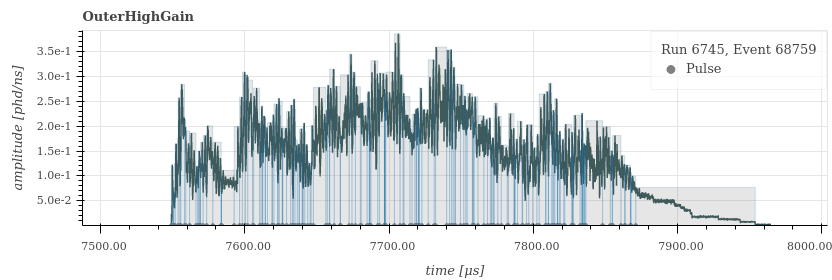
\includegraphics[width=\linewidth]{Figures/OD_Backgrounds/noise_pulse.png}
  \caption{High noise period.}
  \label{fig:noise_od_waveform}
  \end{subfigure}
  \begin{subfigure}{\textwidth}
  \centering
  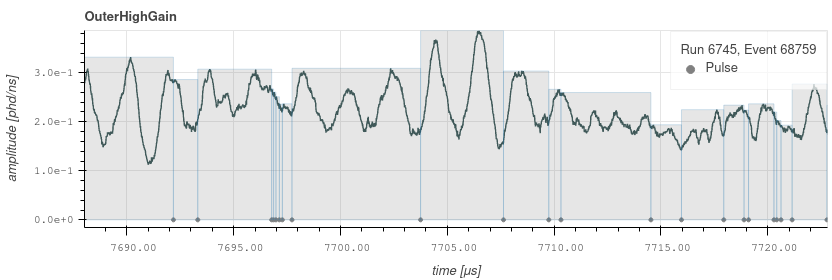
\includegraphics[width=\linewidth]{Figures/OD_Backgrounds/noise_pulse_zoomed.png}
  \caption{High noise period zoomed}
  \label{fig:noise_od_waveform_zoomed}
  \end{subfigure}
  \begin{subfigure}{\textwidth}
  \centering
  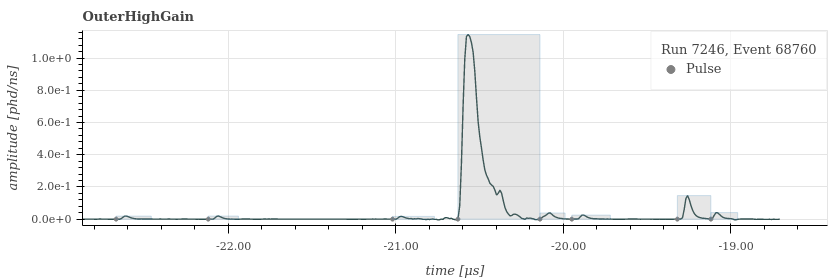
\includegraphics[width=\linewidth]{Figures/OD_Backgrounds/regular_pulse.png}
  \caption{Regular pulses}
  \label{fig:regular_od_waveform}
  \end{subfigure}
\caption{OD summed waveforms showing a noisy period of data and a regular period.}
\label{fig:od_noise_cut_waveforms}
\end{figure}


\begin{figure}[]%
\centering
\begin{tikzpicture}
\centering
  \begin{axis}[%point meta max=150,
    %point meta min=0.0,
    height=10cm, width=10cm,
    view={0}{90},
    ylabel={Pulse Amplitude/Pulse Area},
    xlabel={Pulse Area (phd)},
    xmin=0, ymin=0,
    colorbar,
    colorbar style={ylabel={Count (log$_{10}$}),},
    ]
    \addplot3[
      surf,
      shader=flat corner,
	  mesh/cols=22,
	  mesh/ordering=rowwise,
	  point meta = {z<0.1 ? nan : z}
    ] file {Data/OD_Energy_Scale/noise_cut_2d_low_2.dat};
    
    \addplot3[
      surf,
      shader=flat corner,
	  mesh/cols=30,
	  mesh/ordering=rowwise,
	  point meta = {z<0.1 ? nan : z}
    ] file {Data/OD_Energy_Scale/noise_cut_2d_high_2.dat};
\end{axis}
\end{tikzpicture}
\caption{Representative pulses seen in the OD during SR1.
         No pulse selection has been applied.
         Real events are in the distribution around 0.01 height/area.}
\label{fig:od_noise_cut}
\end{figure}


\par
Using the Random Trigger, the rate seen in the OD was observed for a number of months.
The result of which is shown in \autoref{fig:OD_SR1_Rate} along with the date range used for SR1.

\par
As time progresses the rate of decreases as the OD stabilises.
The various fluctuations in the noise-cut has been linked to the chiller system being turned on, suggesting a grounding failure.
However, as these can be removed with a noise-cut they are not of significant concern.
\begin{figure}[!htbp]
    \centering
   \begin{tikzpicture}
        \begin{axis}[
        date coordinates in=x,
        %xtick=data,
        xticklabel style=
        {rotate=90,anchor=near xticklabel},
        xticklabel=\month.\year,
        xlabel={Date},
        %ymin=247, ymax=250,
        y tick label style={/pgf/number format/1000 sep=},
        extra y tick style={grid=major, tick label style={xshift=-1cm}},
        ylabel={Rate (Hz)},
        date ZERO=2009-08-18,% <- improves precision!
        width=15cm,
        height=6cm,
        ]
        \addplot[smooth, error bar legend,
                 error bars/.cd,
                 y dir=both, y explicit, error bar style={color=orange}] table[x=date,y=noise, y error=noise_error] {Data/OD_Backgrounds/random_trig_rates.txt};
                 
        \addplot[smooth, error bar legend,
                 error bars/.cd,
                 y dir=both, y explicit, error bar style={color=orange}] table[x=date,y=100kev, y error=200kev_error] {Data/OD_Backgrounds/random_trig_rates.txt};
        
        \addplot[smooth, error bar legend,
                 error bars/.cd,
                 y dir=both, y explicit, error bar style={color=orange}] table[x=date,y=200kev, y error=200kev_error] {Data/OD_Backgrounds/random_trig_rates.txt};
                 
        \end{axis}
    \end{tikzpicture}
    \caption{Rate in OD during and before SR1 data taking on a week-by-week basis using the Random Trigger.
    Week -1 corresponds to the month prior to SR1 when the OD PMT gains were higher.}
    \label{fig:OD_SR1_Rate_spare}
\end{figure}
%\par


\begin{figure}[!htbp]
    \centering
    \begin{tikzpicture}
        \begin{axis}[
            title=TODO: Replace with dates and errors,
            xlabel=Data taking week,
            ylabel=Rate (Hz),
            width=15cm,
            height=6cm,
            xmin=-2,
            xmax=14,
            legend style = {column sep = 10pt, legend columns = -1,}]
            \addplot[red, only marks]
                    table [x=Week,y=Rate]
                    {Data/OD_Backgrounds/od_sr1_rate_noise.dat};
            \addlegendentry{Noise Cut};
            \addplot[blue, only marks]
                    table [x=Week,y=Rate]
                    {Data/OD_Backgrounds/od_sr1_rate_100.dat};
            \addlegendentry{100keV};
            \addplot[green, only marks]
                    table [x=Week,y=Rate]
                    {Data/OD_Backgrounds/od_sr1_rate_200.dat};
            \addlegendentry{200keV};
        \end{axis}
    \end{tikzpicture}
    \caption{Rate in OD during and before SR1 data taking on a week-by-week basis using the Random Trigger.
    Week -1 corresponds to the month prior to SR1 when the OD PMT gains were higher.}
    \label{fig:OD_SR1_Rate}
\end{figure}

\par
During the SR1 data taking period, the rate-per-phe is shown in \autoref{fig:od_sr1_rate_vs_threshold}.
Overlaid is the expected rate of backgrounds from \autoref{tab:od_expected_rates}.
Interestingly the observed rate is below what was anticipated.
This unexpected result means that the veto threshold could be reduced to 100keV, which should increase the veto tagging efficiency.
Alternatively, the threshold could be left at 200keV, but the window extended, also increasing the tagging efficiency.

\begin{figure}[!htbp]
    \centering
    \begin{tikzpicture}
        \begin{axis}[
            xlabel=OD Threshold (phe),
            ylabel=Rate (Hz),
            width=15cm, height=8cm,
            xmin=-1, xmax=55,
            ymin=0, ymax=350,
            legend pos=north east,
            grid=major]
             \addplot+[black, smooth, mark=none]
                    table [x=Threshold,y=Rate]
                    {Data/OD_Backgrounds/od_sr1_rate_vs_threshold_smooth_line.dat};
            \addplot[black, only marks, 
                     error bar legend,
                     error bars/.cd,
                     x dir=both, x explicit, error bar style={color=black}]
                    table [x=Threshold,y=Rate, x error=XError]
                    {Data/OD_Backgrounds/od_sr1_rate_vs_threshold_error_bars.dat};
             \addplot[dashed, mark=none, red] coordinates {(0,100) (60,100)};
             \addplot[dashed, mark=none, blue] coordinates {(17.6,0) (17.6,350)};
             \addplot[dashed, mark=none, green] coordinates {(37.5,0) (37.5,350)};
             
             \addplot[orange, only marks, 
                      error bar legend,
                      error bars/.cd,
                      y dir=both, y explicit, error bar style={color=orange}]
                      table [x=Threshold,y=Rate, y error=YError]
                      {Data/OD_Backgrounds/od_sr1_rate_expected.dat};
             
             \legend{,SR1 Data,$<$100Hz Requirement,100 keV (17.6 phe),200 keV (37.5 phe),Expected}                
        \end{axis}
    \end{tikzpicture}
    \caption{Rate of OD backgrounds during SR1 using the Random Trigger. The noise cut has been applied. 100Hz Requirement is for a 500$\mu$s veto window as proposed in \cite{LZ_TechnicalDesignReview_ref}. Expected values are from Table \ref{tab:od_expected_rates}}
    \label{fig:od_sr1_rate_vs_threshold}
\end{figure}

\par
Due to this unexpectedly lower rate, a study was performed in order to understand what backgrounds are (and aren't) being seen.
This is described in the remainder of this section.


\begin{tcolorbox}[colback=red!5!white, colframe=red!50!black, title=Key Plots]
\begin{enumerate}
    \item Simulation Expected Rate of top Components
    \item Scotts Measured GdLS vs Data GdLS
    \item Scaling in X
    \item Scaling justification
    \item Fitted Result
    \item Table of Measured Rates
    \item LCE map?
    \item OD rate over time
    \item R vs Z in background data -> get rock gamma positions    
\end{enumerate}
\end{tcolorbox}


\subsection{Energy Scaling}
\par
When data and simulations were first compared, as in Figure XXX, it became obvious that the light modelling in the OD was significantly different to reality.
Around 50\% of this difference can be accounted for by a mismatch between the PMT gains simulated against those in the LZap reconstruction database.
This effect simply results in smaller pulses and so smaller pulse areas.
However, the remaining difference is not clear where it is coming from, as it would indicate that the LCE is twice what is currently simulated (\autoref{fig:od_lce}).
In the pulse area parameter, this should remain just a linear scaling, though in other parameters (such as number of PMTs receiving light) it may not be linear.

\par
In order to calculate the energy scaling, Th228 data calibration was used. 
In the decay chain (\autoref{fig:decay_chains}), Tl208 has a prominent 2.6MeV $\gamma$. 
There are two simulated sources of this, firstly, from a calibration source, and secondly from the ${}^{232}Th$ cavern-$\gamma$'s as shown in \autoref{fig:cavern_gamma_energy_distribution}.
For cavern-$\gamma$ simulations, the 2.6MeV was extracted using truth information and the resultant phe plotted.


\begin{figure}
    \centering
    
\includegraphics[width=0.5\textwidth]{Figures/Placeholder.png}
    \caption{Number of PMTs contributing to a pulse against the phe of the pulse. Or some similar plot like that}
    \label{fig:OD_coincidence_difference}
\end{figure}


\subsection{Constraints in Data}
\par
Though the exact rate of GdLS is not known, it is possible to constrain some of the components observed.
Notably, decays within the U and Th decay chains where there the second decay has a short enough half-life such that it is within the LZ event window.
This leaves 3-possible decays, summarised in \autoref{tab:od_constrainable_decays_in_data}.
However, in reality only  ${}^{214}Bi \to {}^{214}Po$ and ${}^{219}Rn \to {}^{215}Po$ can be searched for as the interactions from ${}^{212}Bi \to {}^{212}Po$ are close enough together that they will be merged into one pulse.

\begin{table}[!htbp]
    \centering
    \begin{tabular}{c|c|c|c|c|c}
        \multirow{2}{*}{Decay Pair (chain)}                    & \multicolumn{2}{c|}{First Decay}   & \multicolumn{3}{c}{Second Decay}    \\ 
                                                               & Decay    & Energy (MeV) & Decay    & Energy (MeV) & half-life ($\mu$s) \\ \hline
        ${}^{214}Bi \to {}^{214}Po$ (${}^{238}U_{m}$)          & $\beta$  & 3.3          & $\alpha$ & 7.69         & 160   \\ 
        ${}^{219}Rn \to {}^{215}Po$ (${}^{235}U_{l}$)          & $\alpha$ & 6.76         & $\alpha$ & 7.39         & 1800  \\ 
        ${}^{212}Bi \to {}^{212}Po$ (${}^{232}Th_{l}$)         & $\beta$  & 2.1          & $\alpha$ & 8.78         & 0.3
    \end{tabular}
    \caption{Th and U decay chain pairs with half-lives within the LZ event window of 4.5ms. See \autoref{fig:decay_chains} for the complete Decay Chains.}
    \label{tab:od_constrainable_decays_in_data}
\end{table}

\par
The decay pairs can be searched for by looking for pulses which are reconstructed to be close to each other.

These can be searched for by requiring that two pulses be close in time and close in position. 
The time requirement is dictated by the half-life of the second decay.
The position requirement is to reduce the impact of coincident interactions and decays in other areas of the OD.
As the second decay is an $\alpha$ it does not have significant penetrating power so the interaction will be close to where the initial decay was.
The cuts selected were; the noise cut previously discussed, a maximum position separation as defined by the reconstructed position in \autoref{eq:OD_xy_position}.
The time selection

\iffalse
\begin{figure}[!htbp]%
\centering
\begin{tikzpicture}
\centering
  \begin{axis}[%point meta max=150,
    %point meta min=0.0,
    view={0}{90},
    ylabel={Kinetic Energy (MeV)},
    xlabel={Number of Interactions},
    colorbar,
    colorbar style={ylabel={Count}},
    ]
    \addplot3[
      surf,
      shader=flat corner,
      mesh/cols=94,
      mesh/ordering=rowwise,
      point meta = {z<1 ? nan : z}
    ] file {Data/OD_Backgrounds/od_bipo_rate_200kev_2d.dat};
\end{axis}
\end{tikzpicture}
\caption{The relationship between the number of interactions a neutron has in the scintillator and the neutrons kinetic energy when it enters the liquid scintillator volume for neutrons which are 'captured' in the scintillator volume.
}
\label{fig:OD_BiPo_RnPo_rates}
\end{figure}
\fi

\begin{figure}
    \centering
    
\includegraphics[width=0.5\textwidth]{Figures/Placeholder.png}
    \caption{Rate of BiPo and RnPo decays during SR1.}
    \label{fig:OD_BiPo_Rate}
\end{figure}

\par
One of the difficulties in constraining the rates is that the ~8MeV $\alpha$'s in the chains lie in the region where the OD-trigger becomes active.


\subsection{Position Reconstruction}
\par
For any pulse it is possible to reconstruct the location of the interaction that caused the pulse by a weighted average.
This was performed using a simple weighted distribution (\autoref{eq:OD_xy_position});

\begin{equation}
    x = \frac{\sum{\text{Ch}_{\text{phe}} * \text{Ch}_\text{x}}}{\sum{\text{Ch}_\text{phe}}} 
\label{eq:OD_xy_position}
\end{equation}
Due to limited pre-SR1 calibrations, an insufficient variety of calibration sources were used at varying x-y-z positions in order to adequately determine the resolution of this approach, but it is something a future calibration campaign may be able to tackle. 
However, this provides an insight not-thought possible based upon optical simulations.


\begin{figure}[!htbp]%
\centering
\begin{tikzpicture}
\centering
  \begin{groupplot}[%view={0}{90},
    group style = {group size = 2 by 3,vertical sep=1.5cm,
                   horizontal sep=1.5cm},
                   height=8cm, width=0.5\textwidth]
    \nextgroupplot[
            title=Pulse Area,
            ylabel=Rate (Hz),
            xlabel=Pulse Area,
            width=\textwidth,
            height=6cm,
            %xshift=0.5\textwidth,
            xmin=0, xmax=2000,
            ]
            \addplot [blue] {rnd};
            
    \nextgroupplot[group/empty plot]

    \nextgroupplot[title=All pulses,
            xshift=-0.25\textwidth]
            \addplot [blue] {rnd};

    \nextgroupplot[title=Region 1,
                  xshift=-0.5\textwidth,
                  yshift=1cm,]
            \addplot [blue] {rnd};
    
    \nextgroupplot[title=Region 2]
            \addplot [blue] {rnd};
                   
    \nextgroupplot[title=Region 3]
            \addplot [blue] {rnd};
   
  \end{groupplot}
\end{tikzpicture}
\caption{Position Reconstruction of pulses from various regions in pulse area space defined in the top plot. 
         Each pulse has had the noise cut applied and the position reconstructed using \autoref{eq:OD_xy_position}.}
\label{fig:od_backgrounds_position_reconstruction}
\end{figure}

\par
There are two noticeable features in \autoref{fig:od_backgrounds_position_reconstruction}, firstly at both energy regions reconstructed, a majority of events occur in the top and bottom of the OD. 
Secondly, in (+x,+y) there is a higher rate than in the other tanks.
By labelling the SATs with letters A-D starting from (+x,+y) and going around clockwise, we can try an understand this difference.
Using this labelling, over the period of SR1, SAT A has a rate in excess of 8\% higher than any of the other tanks, with SAT B seeing the next highest rate.
Both SATs C and D saw an equivalent rate.
In \autoref{fig:OD_conduit_geometry}, the SAT placement are shown along with the conduits.
SAT A and SAT B are the only tanks which are obstructed by a single conduit, additionally both tanks cover an entire BAT and TAT. 
The CSD-ports and the OCV legs block the other SATs from the TATs and BATs.
These two effects combined explain the increase in rate seen in SAT A and B.


\begin{figure}[!htbp]
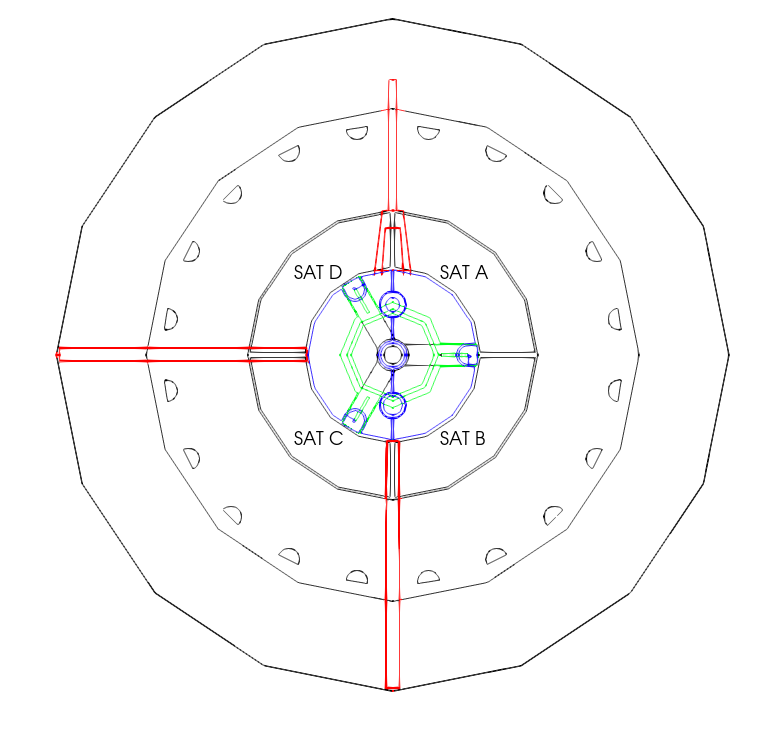
\includegraphics[width=\textwidth]{Figures/Geometry/geometry_with_conduits.png}
\centering
\caption{LZ geometry schematic. The OD geometry excluding the BATs and TATs is shown in black. The BATs and bottom on OCV are shown in green. The TATs, CSD ports and PMT conduits in blue. The DD calibration conduits and the High-Voltage feed through for the TPC are shown in red.}
\label{fig:OD_conduit_geometry}
\end{figure}



\par
As can be seen in \autoref{fig:od_backgrounds_position_reconstruction}, events reconstructed to be at the top and bottom of the OD dominate everywhere.
This supports both \autoref{tab:od_expected_rates} and \autoref{fig:OD_estimated_background_rate} ( \autoref{sec:simulated_od_requirements}), where Cavern-$\gamma$'s are expected to be the largest contributor with the largest contribution coming from the bottom.


\par
As a way of suppressing cavern-$\gamma$'s, a slice of events reconstructed to be in the middle of the side tanks was taken.
The resultant pulse spectrum is shown in  \autoref{fig:od_data_pulsearea_middle_tank}.
What is interesting is that two additional features have appeared.


\begin{figure}[!htbp]
    \centering
    \begin{tikzpicture}
    
    \begin{axis}[
        xlabel=Pulse Area,
        ylabel=Rate (Hz/5phe),
        width=15cm, height=10cm,
        xmin=0, xmax=800,
        ymin=1e-4, ymode=log,
        legend pos=north east,
        grid=major]
            
        \addplot[only marks, mark size=0.5pt] 
            plot[error bars/.cd, x dir=both, x explicit]
            table[x=pulsearea,y=rate,x error=x_error, y error=y_error]
            {Data/OD_Backgrounds/od_data_pulsearea_middle_tank_binwidth_5.dat};
            
        \end{axis}
    \end{tikzpicture}
    \caption{OD pulse area spectrum from pulses reconstructed to the middle of the OD side tanks.}
    \label{fig:od_data_pulsearea_middle_tank}
\end{figure}


\subsection{Fit}
\par
Given the mitigation processes described in \autoref{sec:od_construction_sec}, the contamination is likely to be minimal everywhere. 
Additionally, given what can be seen in Figure XXX, the improved GdLS purification appears to have worked.
As the GdLS came from the same batch produced at Brookhaven as used in DayaBay it is reassuring that it matches closely what was seen there

\par
Instead, what is likely to have happened is that \cite{KamLAND_LS_contaminants_ref}.

\par
Another source, ${}^{7}Be$, which has been considered in fits from similar experiments has been excluded here.
This is because the neutron


\subsection{Cavern-$\gamma$'s}
\par
As discussed in \autoref{sec:cavern_gamma_generator}, the $\gamma$'s from decays within the rock are of significant concern.
blah blah blah...
Over the continued course of the experiment it will be interesting see if an annual modulation is observed such as that in \cite{cavern_gamma_annual_modulation_CoGeNT_ref, cavern_gammas_in_Soudan_mine_ref} as it may be a more significant background for LZ than previously considered.